\chapter{如何改善} % Introduction chapter suppressed from the table of contents

\hypertarget{ux654fux6377ux5f00ux53d1ux8fc7ux7a0bux6539ux8fdbux6848ux4f8b}{%
\subsection{敏捷开发过程改进案例}\label{ux654fux6377ux5f00ux53d1ux8fc7ux7a0bux6539ux8fdbux6848ux4f8b}}

\hypertarget{ux6708}{%
\subsubsection{5月}\label{ux6708}}

A公司一直为某电信公司专门提供客服、线上播放等IT业务。\\
张工是公司的中层管理者，管理好几个开发团队，有5位项目经理向他汇报。\\
他听说老同学的团队都开始用敏捷开发，很感兴趣，便参加了几次敏捷交流会，觉得可以解决很多开发团队的问题，尤其是可以快速交付给客户。\\
他便提建议给部门经理推动敏捷开发，找咨询公司做相关培训，例如SCRUM
Master内部培训，然后全面开展实施。\\
开始时，部门经理有些怀疑，问：``听起来很吸引，但后面那些工程文档都不做，会不会影响质量和交付？客户都是专业做电信的，不缺钱，但是对质量要求很高。''\\
张工解释说：``只要利用敏捷把过程变成迭代，快速交付、改善工程的问题不难，主要是人的问题。''\\
部门经理听到敏捷可以比以前更快速交付，因之前客户经常抱怨项目延误，他也希望可以改变，就答应了。

\hypertarget{ux6708-1}{%
\subsubsection{8月}\label{ux6708-1}}

开发组长王工，三十出头，毕业后一直做开发，一年前晋升为组长。周五下班后与朋友喝酒，很开心地说：``太兴奋了。我们团队刚参加了两天SCRUM
培训，并指出我们以前按传统瀑布式开发的种种问题。我们会两周一次迭代并割接上线，还会与用户代表定期交流，不再会像以前几个月交付后才发现开发出来的功能不合需求。\\
现在团队合作不像以前只按工种工作，也会跟产品经理、业务方面更充分合作，给客户带来更高价值。\\
工作方式也会改变，以前要写需求规格说明书，现在简单化成产品需求卡片，以前我们要做详细项目计划和甘特图。现在会改成用燃烧图和``KANBAN''。
每天用便利贴去写要开发什么内容贴在白板上面，我们会改成叫SCRUM
Team。工作区周围都有SCRUM的海报，提醒我们SCRUM的重点。团队也没项目经理了，自己管理自己。部门经理会变成产品负责人，敏捷开发方式让我们团队自己做决策，不仅仅是技术方面，项目相关的也由我们项目组一起讨论决定。''\\

\hypertarget{ux6708-2}{%
\subsubsection{9月}\label{ux6708-2}}

王工的朋友老杨周五晚喝酒时问他：''你们团队使用敏捷SCRUM后，效果如何？''\\
王工立马面露笑容，充满自信地跟大家说：``我们培训后就使用SCRUM的方法，每2周一个冲刺，每次冲刺前都会用故事点来估算每个功能多大，然后按本次冲刺的资源，估计可以完成多少功能。然后用看板来监控模块完成的情况，哪些正在开发中？哪些已经完成？团队和管理者都可以一目了然，不用像以前......。''\\
``听你这样说，我也要尽快提议领导引入敏捷开发。''\\
``我还未说完，我们每天早上也按照SCRUM的规定站立会议，每人说自己完成了哪些任务，今天做什么......。''

\hypertarget{ux6708-3}{%
\subsubsection{10月}\label{ux6708-3}}

喝酒时老杨问王工：``你们项目如何？''\\
王工听完，没有立马回应，把注意力放在窗外的大街上，想了一下，然后说：``我们本应上周要完成一次冲刺后的割接上线，但被推到下次了。''\\
``为什么？''\\
王工说：``我们按培训学到的做冲刺计划会议，按照产品的待办事项列表，团队利用扑克牌一起估算每一事项所需要的时间。我们总共8位开发人员，其中有一半是刚毕业不久，但大家刚上完培训，很有信心，虽然技术主管张工对我们的估算有些顾虑，觉得我们太理想，但大家刚培训完敏捷，张工也希望让部门经理尽快看到敏捷开发可以加快速度，我们就按这`进取式'估算开展两周冲刺。但因新人多，编码水平有限，虽然大家已经尽快把开发出来的代码交给系统测试人员手工测试，依据测试发现的缺陷修正再测试，但割接上线期限前4天还有很多Bug没改好，最后3天，基本是天天加班，最终到上线期限仍然有不少问题，最终割接前测试，还是不能达到客户要求的水平，没办法上线。大家确实都尽力冲刺了，但未能达到我们本来希望的结果。''\\
``你们开发人员在提交代码到系统测试之前，有没有自己先自测？''\\
王工说：``我们敏捷开发每天早上站立会议上都用看板，记录每个模块的进度完成情况，开发编码人员都说自测过。''\\
``如果开发人员能自己把握好交付代码的质量。不应该等到系统测试才发现这么多问题要解决。你们团队是怎么做自测？有记录吗？''\\
王工说：``这我就没有详细问了，因为我们学完SCRUM后，大家更关注开发速度，用看板保证按计划的进度，不延误。但没想到后面缺陷会这么多。而且有些问题改完以后还会导致另外一些Bug发生。到了最后，因为赶时间，大家对修改Bug已经麻木了。''\\
``你们之前不是都有代码评审和扫描的习惯吗？''\\
王工说：``之前我们确实比较多评审，除了评审核心设计和代码，我们还要求组长抽查新人开发的代码，并且要求提交代码前必须通过扫描。但我们为加快速度，没有硬性要求必须先通过扫描。经你一问，我想这也可能是出现很多Bug的原因之一。''\\
``你们有没有事后迭代复盘？复盘可以帮团队分析之前有哪些不足，后面改进。''\\
王工说：``我们都交付不了，哪里有心情来做回顾、复盘。最后几天冲刺，大家每天都没睡好，大家都只想回去好好睡一觉。''\\

\hypertarget{ux6708-4}{%
\subsubsection{11月}\label{ux6708-4}}

部门经理之前收到客户总监电话，投诉一些技术缺陷，导致好几次不能按计划上线，问为什么正在交付的软件质量变差了？\\
张工被问到是什么原因时无法回答，只能说立马回去探索原因，尽快汇报。\\
张工从部门经理办公室出来后，找其中一位项目经理李工喝茶，问他对今次敏捷改革的意见。\\
两人都赞同敏捷开发应能帮助团队提升，当张工问李工有什么可以改善的地方，李工说：``让团队自主是件好事，但因为我们专注做这块业务已经很多年了，本来业务的变化不多，只是一些功能微调，所以开发人员尽量不去修改核心代码，怕改动了反而会影响投产，无法切割。为了不触及原始代码，新代码都只能在核心的外围去写，但这种做法效率很低，无法有效长久维持，到时会被迫重写整个产品。而且懂老代码的开发人员大部分都离开了，代码维护越来越困难。\\
敏捷教练强调团队自主管理，给团队空间发挥。但SCRUM的教练缺乏软件工程的基础，只懂项目管理过程。所以他们也解决不了软件相关的问题。只是把精益管理怎么做迭代、怎么做回顾这些基本过程再解读一下，解决不了实际问题。''\\
张工说：``很赞同，这是必须要解决的问题。但现在燃眉之急是要解决主管提出的客户投诉不能按时交付这紧急问题。不然我们以后也不敢再提敏捷开发了。''\\
无论张工或李工也没有能去总结出什么好的解决方案。现在推行敏捷才刚刚3个月，绝不能打退堂鼓，回到本来的状态。但应怎么解决敏捷带来的问题，挽回部门经理与客户的信心呢？\\
:= = =
从上面案例看到，本来管理层希望利用敏捷开发，加快软件开发的交付、减少延误、令客户更满意。但因为只注重项目进度是否延误，没注意如何改善软件开发本身的质量，也因为团队成员能力不足，开发出来的软件缺陷比以往还多，导致后面大量返工，恶性循环，后面更导致延误和客户投诉。\\
因为以往没有关注软件的设计与维护，导致软件难以修改，开发人员都不敢改动任何代码，怕可能会引起系统崩溃。\\
问题出在哪里？是否不应采用SCRUM这种敏捷开发方法？\\
敏捷开发有多种方法(SCRUM只是其一）。\\
因为张工的团队不仅仅要管好项目进度，也要确保软件产品的质量。SCRUM只包括项目管理部分，不全面。\\
是否加上其他敏捷开发方法，如极限编程(XP eXtreme
Programming)便可？（因它的发明者Kent
Beck本身是一位精通面向对象的编程员，所以XP不仅仅关注项目管理，也包含编程的最佳实践。）\\
想避免张工这些问题再发生，就要系统地解答以下问题：问题出在哪里了？那些敏捷开发的实践没有做好？\\
首先要清楚有哪些敏捷开发的实践。虽然敏捷宣言已经有超过20年历史，也越来越多开发团队使用敏捷，但敏捷这个词却越来越被泛滥使用。如果你细问某使用敏捷开发的团队，可能发现他们只是每天站立会议和规定每四周发布。就算一些使用SCRUM的团队，也像张工情况一样做过培训，团队也不一定全部按照SCRUM的实践执行。Ken
Schwaber，《Scrum Guide》的作者之一，说大概七成企业不是完全依据Scrum
Guide，都只是挑选某部分执行。\\
针对缺乏完整的敏捷实践，幸好Michael
Neumann在2022年先搜索2010年到2021年期间关于软件开发实践的资料，再从搜索得出的867篇筛选，按是否与软件开发和敏捷实践相关、有没有经过同行评审、是否是英语、是否少于3页等条件，最后选出37篇文章和书籍（例如包括
《Scrum Guide》, 《XP
Explained》），最后从里面的关键字得出综合敏捷实践列表，我按出现频率最高（85\%）做出表1-1：\\
%\url{文件:敏捷开发实践汇总列表1-1.jpg}

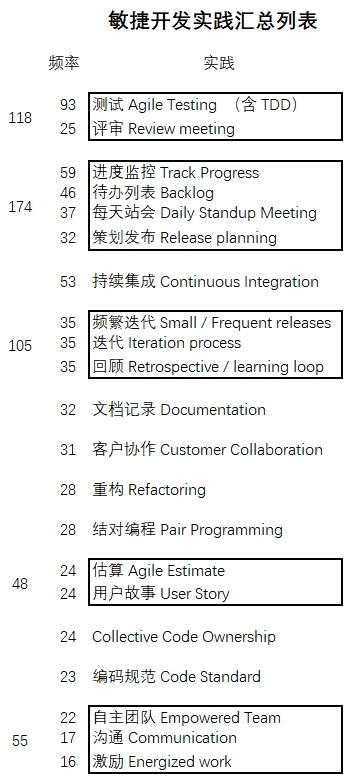
\includegraphics[width=10cm]{敏捷开发实践汇总列表1-1.jpg}

表1-1

注释：频率是在37文件里总共出现次数，这列表的总频率是719，原本完整列表的总频率是840，占85.6\%。

\hypertarget{ux5982ux4f55ux6539ux5584}{%
\subsection{如何改善}\label{ux5982ux4f55ux6539ux5584}}

谈如何依据敏捷实践列表来解决张工的问题前，必须先抓到重点。这么多敏捷开发的方法、框架，最关键和重要是哪些实践呢？\\
先邀请进入培训室，听我给学生讲的第一堂课。\\

\hypertarget{ux7b2cux4e00ux5802ux8bfe}{%
\subsection{第一堂课}\label{ux7b2cux4e00ux5802ux8bfe}}

``先问你以下关于汽车公司的问题：''



\framebox{%
\begin{minipage}[t]{0.97\columnwidth}\raggedright
CompT vs CompG

\begin{itemize}
\tightlist
\item
  1955年前后,生产一辆汽车的成本:CompT成本=CompG成本x2
\item
  全球销售额:CompG 销售额=CompT销售额x140
\item
  平均每个员工年汽车生产量
\end{itemize}

%\url{文件:T和G图1.jpg}

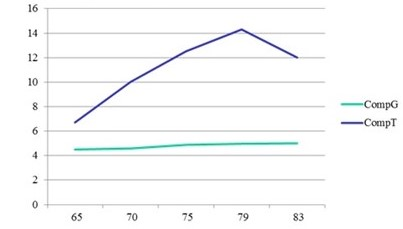
\includegraphics[width=10cm]{T和G图1.jpg}

图1-1

``T公司在60年代，在销售、生产成本都远远不如G公司，但它每年生产率都一直提升。请猜猜T和G是那家公司？
（提示：两家都是世界级汽车公司，现在你还能买到它们生产的汽车。）''\\
``从图看到G公司平均一个人生产汽车的数量，从六十年代到八十年代，一直都没有超过6辆，但是T公司就到八十年代超过14辆。''\\
``T是日本丰田，G是美国通用。''\\
\strut
\end{minipage}}


为什么丰田汽车能从一家在战后本来快破产的小公司，可以超越那些美国的巨人公司，如通用、福特等，成为世界上最大的汽车公司呢？\\
我们在说这个之前，首先要了解汽车生产的历史，汽车发明之初属于小众的玩意，需要定制生产，所以非常昂贵。之后福特先生使用了工业生产的生产线概念，大规模大量生产汽车，把汽车的平均价位降到中等家庭可以负担的水平。

\framebox{%
\begin{minipage}[t]{0.97\columnwidth}\raggedright
福特 Model-T\\
它是第一辆一般人买得起的汽车。首辆现代汽车是由德国奔驰(Benz)于1885制作，但是这些第一代汽车都非常昂贵。\\
老福特是一名工程师，对机械特别感兴趣，白天是爱迪生公司的总工程师，到了下班后就研究汽车发动机。经过10年的不断优化，最终开发出4冲程自动汽车发动机，他的发明大大降低了汽车组件的成本。1908年Model-T首次推出市场，售价是850美金，虽然已经比同期的其他厂家汽车便宜，但还是超出一般工人家庭可以负担的水平。\\
为了进一步降低成本，老福特觉得必须想其他办法。汽车组装一直都是作坊式运作，所以组装汽车需要超过12个工时。为了降低组装时间，必须要学其他工厂，如啤酒厂、面粉厂，它们都已经是流水式生产线生产(Assembly
Line)。福特把整个Model-T组装拆分成84步骤，并培训工人只做一项工作，
还聘用了工程顾问
Taylor先生设计整个流程，提高效率，最终可以一个半小时完成组装一辆汽车。\\
生产线生产帮助福特公司把成本和售价降下来，在15年期间（1913
\textasciitilde{}
1927），福特公司总共生产了15,000,000辆Model-T。虽然大量生产能直接降低生产成本,但这种做法也要付出代价：

\begin{itemize}
\tightlist
\item
  为了生产所有都是同一个款式同一个颜色，黑色
\item
  为了提高生产的效率，也增加了组件的库存量（为了提高效率、降低成本，大部分组件都要批量生产(Batch
  production)，例如轮胎。从右下图看到工厂里存在大量轮胎。)
\end{itemize}

%\href{文件:FordModelT_2023-06-10_100431.jpg}{600px}


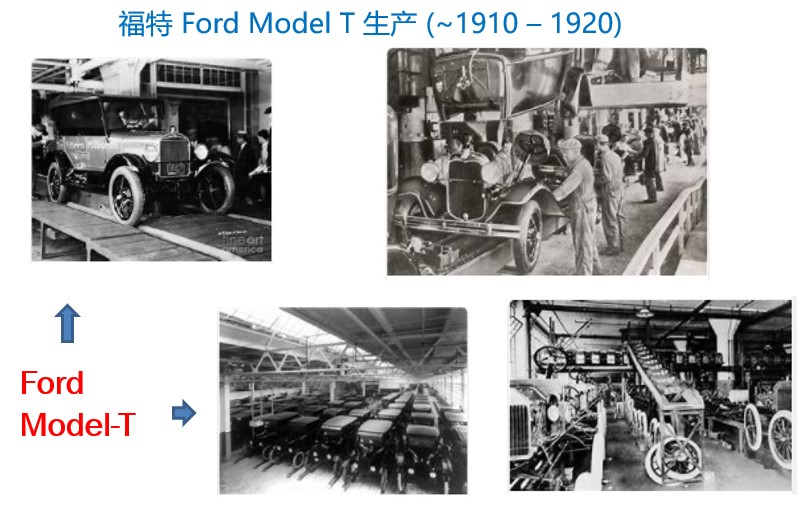
\includegraphics[width=10cm]{FordModelT_2023-06-10_100431.jpg}

图1-2

\strut
\end{minipage}}

\textbf{Federick Taylor 与科学管理(Scientific Management)}\\

\framebox{%
\begin{minipage}[t]{0.97\columnwidth}\raggedright
十九世纪末美国很多工业快速扩张，Taylor先生发现当时很多工厂生产力很低，例如钢铁厂。他是很落地、实干的人，就想有什么好方法可以提高生产力，工人也多赚些钱。他发现很多工作都未设计好，未能好好利用工人，他针对工作本身做很多科学研究，测量每个工作应该多长时间，怎么做最好，然后按他的最佳设计把工作细分，也同时要求公司提高员工的奖励，希望工人看到因科学管理，提高生产，个人也受益。1890年，他加入了Bethlehem
Steel------钢铁业的大公司，帮它设计了很多奖励制度，也设定了一些叫工业工程师(Industrial
engineers)岗，发现生产力可以提升30-40\%。后来公司被收购，他也被辞退，便去做顾问。当时都没有顾问这个职业，他可算是全球首位工程顾问。
\strut
\end{minipage}}


\hypertarget{ux4e30ux7530ux6545ux4e8b}{%
\subsection{丰田故事}\label{ux4e30ux7530ux6545ux4e8b}}

二战后50年代,丰田汽车规模很小，经营很困难，在破产边缘。
但丰田创始人喜一郎先生明白美国生产线的弊端，意识到未来的汽车生产必须是Just-In-Time(JIT)：

\begin{description}
\tightlist
\item[]
\textbf{JIT =
每个工作步骤所需配件按生产需要到达（不晚到也不早到），把生产过程中的配件降到零}
\end{description}

\begin{itemize}
\tightlist
\item
  每一辆都是按客人订单订制：例如颜色、配置、左右钛等
\item
  从钢材原料开始，整个生产线零等待、零浪费
\end{itemize}

\hypertarget{ux8fdcux666f-vision}{%
\subsubsection{远景 Vision}\label{ux8fdcux666f-vision}}

\begin{itemize}
\tightlist
\item
  0 defect零缺陷
\item
  100\%value added百分百的增值
\item
  One-piece flow, in sequence, on demand
  按订单的流水线生产，过程中零浪费
\end{itemize}

喜一郎先生安排总工大野耐一先生去美国汽车公司考察。

总工大野耐一先生从美国的超市（非汽车公司）得到如何做Just-In-Time的启发，回国后就开始在丰田全力推动。开始时，很多人都觉得Just-In-Time
这个愿景好像是远不可及的梦想。而到了今天，现代汽车生产都基本做到了当年喜一郎先生和大野耐一先生的JIT梦想。（详见附件``现代汽车生产''）

为什么丰田可以超越西方的巨头汽车公司？不会是日本人比欧美人更聪明吧？会不会是有很多新的技巧？比如看板那些方式。但欧美的汽车公司也不是傻瓜，他们会模仿。所以要了解为什么日本丰田公司能超越，并行成了如今的一些全球生产线标准，就得了解丰田背后的系统。\\

\hypertarget{ux6c34ux9762ux4e0bux7684ux7ba1ux7406ux601dux8def}{%
\subsection{水面下的管理思路}\label{ux6c34ux9762ux4e0bux7684ux7ba1ux7406ux601dux8def}}

%\url{文件:冰山.png}


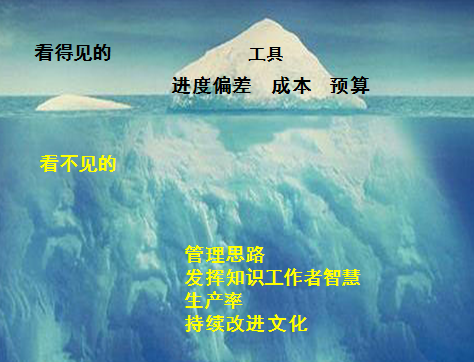
\includegraphics[width=10cm]{冰山.png}

图1-3

为什么丰田能成功地把汽车生产做到 Just-In-Time
，超越西方的巨头，使日本汽车制造过程成为世界``标准''？\\
但我们不能单从表面看这``系统''的方法和技巧，例如大家都熟悉的看板管理（他的竞争对手通用、福特肯定都学过），更重要是了解背后的管理思路。我们看看下面丰田七个习惯，开始了解水面下的``系统'':\\
\# 容易实现的目标不是好目标

\begin{enumerate}
\tightlist
\item
  不以``我们公司''作主语
\item
  重复五遍``为什么''
\item
  持续改善没有停止
\item
  成长比成功更重要
\item
  以忙碌为耻
\item
  从心里相信``大家的力量''
\end{enumerate}

\hypertarget{ux5bb9ux6613ux5b9eux73b0ux7684ux76eeux6807ux4e0dux662fux597dux76eeux6807}{%
\subsubsection{容易实现的目标不是好目标}\label{ux5bb9ux6613ux5b9eux73b0ux7684ux76eeux6807ux4e0dux662fux597dux76eeux6807}}

\textbf{\texttt{不是“削减一成”，而是通过“取消一个零”来发现浪费}}

``如何把原先需要3小时的工作，改用3分钟完成''\\
如果听到上司以上要求，你该怎么回答呢?如你回答：``这太强人所难了''、``绝对做不到''，请读以下丰田故事。\\
汽车生产线不可能只生产一个型号的汽车，但要生产线上面的机器改变配置，从生产某个型号到另一款，通常需要更换的时间长达2-4个小时，必须要尽量压缩更换时间，才能提高生产效率。所以丰田工程师在大野先生指导下，开始研究如何可以压缩更换时间。他们发现装置更换包括2类：\\
\#内部装置更换，必须要在机器停下时更换

\begin{enumerate}
\tightlist
\item
  外部装置更换，可以在机器运转过程中进行更换
\end{enumerate}

因此，要缩短时间，就要把2种更换分开，尽量用外部替换的方式。同时对内部和外部的装置替换进行改善，最终可以把更换的时间压缩到一个半小时。工程师给大野先生汇报改的是经过4个月不断摸索和试验的结果，原本以为大野先生会很满意，但大野先生说：``既然能缩短到现在的水平，如果你们继续改善，时间应该能压缩到3分钟。''改进组大部分人都觉得做不到，但其中一位资深工程师说：``如果我们能想办法把所有内部装置改为外部装置，3分钟也不是不可能。''改进团队就按这个思路开始做改革，同时研究各种切割工具、模具，并且减少多余操作，尽量用一个动作就能完成所有更换。通过5个月时间，做了超过100轮改善，最终达到了大野先生定下的目标。\\
容易实现的目标不是好目标，丰田这个原则能否也用于我们软件开发的过程改进呢？\\
学员：应该也可以吧。\\
我：是的。比如希望减少后面在验收或者最后系统测试发现的缺陷数，我们的目标就不应该仅仅是降低5\%、10\%这种没意义的小变化。你估计可以定多高合理呢？\\
学员：最多降个25\%到30\%。\\
我：不。从我们实际操作的例子来看，如果他之前没做过过程改进的话，在做过几轮迭代后，缺陷数能达到减半是很正常的。例如本来完全没有做正态代码扫描，后面增加了这个检测，或者本来没有注重代码人员自己做单元测试，后面做了，通常都能把后期的缺陷减半。如果不能减半的话，管理层是没有兴趣继续支持这种过程改进的。做培训、监控等着投入成本也不小，如果没有可观的回报，肯定高层会叫停，持续不下去。大部分软件开发公司，因为缺乏数据、度量，很少有标杆的概念，但也不是全部。尤其是客户对质量有要求的公司，比如证券、银行、保险这些软件公司，开发经理会问标杆这个问题。从他们开始关注标杆，就会了解到管理层对持续改进、度量或者提升等，都有一定要求。大家对质量或者生产率、工作量等，都会有具体的提升要求，并定期监控。公司才会提高本身的竞争力，不会很容易被淘汰。\\
如果大家针对每次迭代的系统测试缺陷密度都进行统计，就可以开始建立团队的内部标杆或者基线，作为后面的参考。日后在做项目估算的时候，便可以依据以往的历史数据，更准确去做好新一轮迭代的策划和估算。\\
这个思路也不仅是用在缺陷，也可以用于工作量、工期等的估算。\\
刚刚说的只是其中一种标杆管理，除了参考团队自己的以往数据和趋势，也应该可以在公司内部与其他团队比较，或者和公司的主要竞争对手比较，例如找行业中最优秀的公司去对比，就会知道自己的不足。\\
丰田一般会选行业里最强的对手作为基准（标杆）。例如，1965年，美国通用汽车公司是世界顶尖。例如销售额的规模，丰田与通用是1:60，完全不在同一个层次上。成本上丰田对通用是1:0.5，成本是通用的两倍。\\
丰田把当时顶尖的通用公司当成了自己进行标杆管理的对象。丰田就思考怎么激发内部去改善。例如，同一个零件的成本在丰田是一千日元，而通用的成本是四百日元，丰田就会用四百日元作为成本基准，把差额六百作为不必要花费，要求团队立马改善，尽量想办法达到标杆。\\

\hypertarget{ux6807ux6746ux7ba1ux7406-benchmarking}{%
\paragraph{标杆管理
(Benchmarking)}\label{ux6807ux6746ux7ba1ux7406-benchmarking}}

很多公司都会用百分比来设定改善目标，但改善了百分比，不一定代表质量有改善，例如某快递公司去年送包裹未按时送达占8\%，今年是6\%，好像已经改善了2\%。但去年托运的数量是500万件，所以8\%是40000件。今年的数量是750万件，所以今年的6\%就是45000千件。所以今年包裹延误增加了5000，这样非但没有任何改善，反而服务变得更差了。所以更重要是看数字本身。\\
丰田（如下图）很注重各种标杆，例如内部标杆、竞争性标杆等。软件开发也应该同样利用数据来制订量化目标。\\
%\url{文件:丰田p1.png}



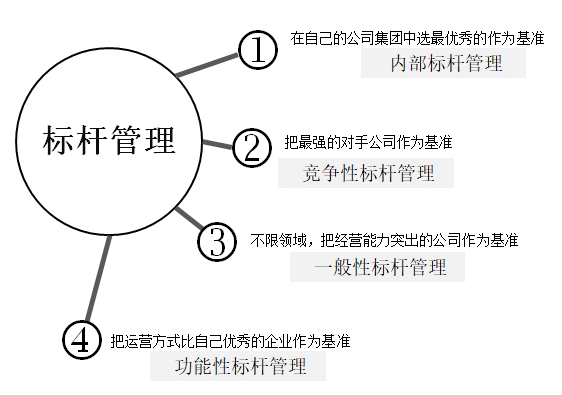
\includegraphics[width=10cm]{15页替换图片.jpg}

图1-4

（图1-4参考岩松义人的《为什么是丰田》）

\framebox{%
\begin{minipage}[t]{0.97\columnwidth}\raggedright
某家专门开发金融软件产品的公司：

研发总监问我“你接触这么多国内的企业，觉得有哪家优秀的，可以作为我们的标杆？ 我们尝试寻找，但还未找到。有些优秀的公司，但它们业务跟我们不同，我们产品是面对企业，也非嵌入式软件（我们不生产硬件）。”\\
“确实难找，我真没遇到过，但为什么你只看国内公司？” 
\strut
\end{minipage}}

从以上对话看到越来越多高水平开始用标杆管理，但标杆必须是比自己高很多才有作用。

\hypertarget{ux4e0dux4ee5ux6211ux4eecux516cux53f8ux4f5cux4e3bux8bed}{%
\subsubsection{不以``我们公司''作主语}\label{ux4e0dux4ee5ux6211ux4eecux516cux53f8ux4f5cux4e3bux8bed}}

\begin{itemize}
\tightlist
\item
  不是从``专业''的角度，而是从``顾客''的角度生产产品
\end{itemize}

\begin{description}
\tightlist
\item[]
创业大忌------闭门造车,所以丰田的原则，对客户有用就一定做出来，但对客户无用或者不想要，就绝不生产\\
\end{description}

有些汽车公司技术很厉害，主要精力用于做到技术领先。但丰田的原则是，如果对客户有用就一定要做出来。因为如果不是以客户的需求为主导，就很容易导致生产出来的产品，并非客户所需要的。\\
例如宅急便是一家日本专门送货搬家的公司，他们发现市场上的送货车不方便驾驶员使用，便提出要求配送车应该便于装卸货物，且方便驾驶员上下车，也易于在车装卸区上下工作。例如，让驾驶员在车里可以直接从座位走到后面的货物区进行操作。一般汽车公司听完这种特殊要求，就会反驳说你们不熟悉汽车设计，这种奇怪的设计违背了很多汽车设计的原则，整个车的架构不稳定，且会更耗油，建议你还是用我们这种标准设计好的送货车，而且价位也合理。
而当丰田听完这个需求，却说如果你们觉得有这个需要，我们的工程师就跟你一块设计能满足你们需求的车。后面确实为宅急便公司生产出了合适的送货车。\\
丰田汽车确实在汽车行业比竞争对手更灵活，更尽量满足客户的个性化要求。
其他汽车公司虽然嘴上说``一切为了客户''，但总是想生产能让公司标榜最新技术的车型，最终还是主要考虑企业的利益。\\
必须从``顾客''的角度看，不单从工程师的视角看------这不仅适用于汽车制造,在软件开发行业也适用，但要平衡，有时候不要误认为客户很清楚自己的要求，因为他们也没有软件开发的经验。例如客户频繁提出的需求变更，因为他们不知道这种频繁的变更，反而会导致软件公司大量返工，对最后能否按时交付有很大的影响。所以软件开发在需求方面永远是优化，尽量花精力去把它做好，不然会影响后面工作。但如何做好，不仅是听客户的需求，并需要以顾问的角度指出客户的误区。

\hypertarget{ux91cdux590dux4e94ux904dux4e3aux4ec0ux4e485-why}{%
\subsubsection{重复五遍``为什么''(5
Why)}\label{ux91cdux590dux4e94ux904dux4e3aux4ec0ux4e485-why}}

最重要的不是追究责任而是找出根因。

五个``为什么''是一种找根因的方法，实例可详见附件``5 Why''：

\begin{itemize}
\tightlist
\item
  不停留在``原因''上，而要找出``真因''，彻底改善
\item
  不追究责任，而是追究原因
\end{itemize}

丰田要求检查人员不仅仅检查过程与结果、做统计报告、交给负责的工程师，也必须分析产生不合格的原因，使同类的问题不再发生。检查人员不仅仅是``考官''，也作为``内部教练''，指导生产的持续改善。反过来，如果下属因出错导致失败，立马被上司骂，觉得很难受，就会从反省变为排斥。如果公司有这种``责难，追究责任''的风气，坏消息就会被隐瞒。所以丰田有一条原则是``Hard
news first （先说坏消息）''。
当工程师找出了问题就必须要求他查找原因、提供数据，但很多时候这个工作并不简单，但大野耐一先生决不放弃，必须找到根因。他说：``做到一半是不行的，只有一个期限------``到完成为止。''

\framebox{%
\begin{minipage}[t]{0.97\columnwidth}\raggedright
帮一家香港公司做软件开发质量改进，公司历史悠久，但公司主业不是做软件开发，而是承担办公楼的机电工程项目，例如电梯、空调、机房或数据中心的建设。
公司管理层大部分就是工程师出身，比较严谨。推动这改进项目的公司高管刘先生说，``我们公司这么多年有一个弊端------员工都是报喜不报忧。如果有什么成功案例是都会尽力在公司内宣扬，但是有什么错误问题出现就绝口不谈，导致很多宝贵的经验教训没有保留下来，供日后参考。''
\strut
\end{minipage}}


\hypertarget{ux6301ux7eedux6539ux5584ux6ca1ux6709ux505cux6b62}{%
\subsubsection{持续改善没有停止}\label{ux6301ux7eedux6539ux5584ux6ca1ux6709ux505cux6b62}}

``请猜猜丰田汽车在90年代初，平均每员工一年提多少条改进建议?"\\
``大概每月一条，12 - 15条。''\\
``老师这样问应不止，多一倍，25条左右。''\\
丰田当时大概8万员工，一年里共有4百万条改进建议，平均每员工每年提50条。\\
丰田某部门在一年半时间，成功地把平均零件替换时间从90分钟缩短到30分钟，但再过了半年会问这几个月只缩短了几分钟，丰田管理者便会问为什么。\\
人有的时候很想``往前跑''，但有的时候也想``停下来休息''。对丰田而言，比起以为``已经胜利了''而在睡午觉的兔子而言，他们更推崇不倦不怠一直向前进的乌龟。\\

\framebox{%
\begin{minipage}[t]{0.97\columnwidth}\raggedright
某家成都的软件开放公司总经理是从日本的回国的，对质量很有要求，开始时，推进了很多质量改进的方式，确实把大量缺陷减少到原来的一半。过了不到一年时间后就没有再持续改进了。当总经理问我是什么原因时，我就会用丰田的故事说明持续改进必须从高层开始，且一直坚持下去。
\strut
\end{minipage}}

所以改善能否成功，大家能否把改进养成习惯，取决于管理者能否坚持
，不单是依赖学到什么技巧。

\hypertarget{ux6210ux957fux6bd4ux6210ux529fux66f4ux91cdux8981}{%
\subsubsection{成长比成功更重要}\label{ux6210ux957fux6bd4ux6210ux529fux66f4ux91cdux8981}}

\begin{itemize}
\tightlist
\item
  要培养人才，``改变体制''比``改变人''更有效。\\
\end{itemize}

有些工厂只依赖张贴标语、海报，希望可以减少工地的事故发生率，但丰田不注重喊口号，而是动手干实事，包括机械保安、设备保安等。

%\href{文件:ft_223.1.png}{500px}



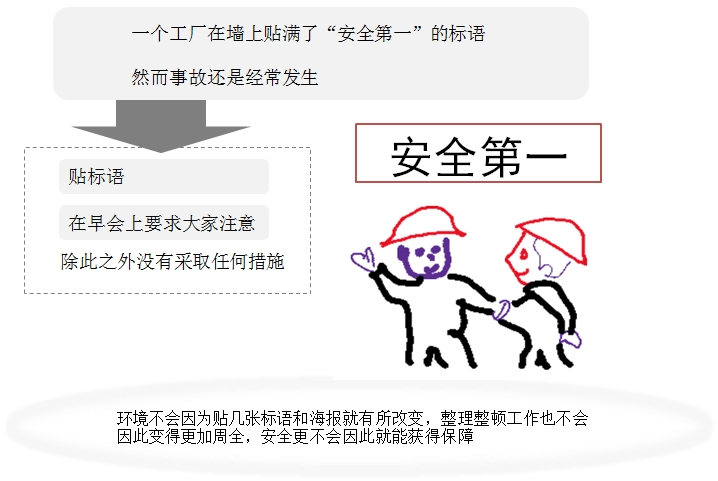
\includegraphics[width=10cm]{Ft_223111.jpg}

图1-5

所谓5S指的是：整理、整顿、清扫、清洁及修养。（详见附件``5S法''）无法做到这些基本原则的企业及个人是无法生产出优质产品。\\
在这些基本原则中,丰田尤其注重``整理和整顿''。\\
``处理掉不需要的东西是整理。使得任何时候都能把想要的东西拿出来的叫整顿。只是把东西放整齐的则叫做排列。我们要求在生产现场必须要做好整理和整顿。''\\
所以如果有机会进丰田的生产场所，你会感觉到很清洁很干净，没有大堆废物或者零件堆在里面，这也直接影响到工作的效率。\\
这种5s的好习惯，其实不仅仅适用于工厂生产，对个人也适用。\\
因为我经常要去客户现场做培训，每次离开的时候都会很仓促，常常遗漏一些小物件，比如充电器等。我就按5s的要求，给每件东西都安排一个背包或者手提袋固定的地方。\\
以前坐飞机时也常常会把一些电子产品(Kindle等)或者耳机遗忘在座位前的口袋。学习了5S后，我都会在下机之前检查一下，确保东西把所有东西放回它的固定位置，后面就没有再遗漏东西了。\\
所以当我在酒店大厅听见前台接到客人电话，说在房间遗漏了iPhone，请前台快递给他，心想5s习惯应该能帮到他。\\
成长不是仅仅按既定方向去做，必须思考动脑筋，并了解背后的目的才能真正取得效果。\\
在七八十年代，汽车公司开始引进自动化机器人提高生产效率。\\
但大野先生对引进机器人是很慎重的，他觉得如果只是觉得机器人用起来很方便，可以替代工人去完成工作，就表示那家公司没有有效的使用机器人，要真正用好机器人，必须让它与工人的工作合拍，辅助工人才有意义。\\
所以丰田不但要求人的工作和机器人的工作要明确分工，并且要2者能和谐的存在。例如丰田当要决定，最后在组装工序中引进机器人，他们工程师都会慎重考虑，要经过很长的一段时间做准备，里面分析如果人会采用什么方式去做？什么工作是机器人做得了，什么是机器人做不了。例如，哪些零件更适合用机器人装配。\\
另一方面，回顾七八十年代的美国通用公司，它就花了很多钱用IT把生产自动化，但最后没有产生什么效果。估计就是因为没有想清楚，为什么要自动化，自动化怎么帮到人的工作并产生效果，只是相信用技术、高科技就能提供生产率。\\
二战后，日本经济萎缩,丰田辞退了不少员工。1950年，朝鲜战争爆发，需要大量增产，但丰田选择了只增加设备，而不增加人手，大野先生也借这机会，完善丰田生产方式，成功找到了以不增加人手为前提的增产办法。\\
这些丰田的成长故事也适用于软件开发团队，例如，有些软件开发团队盲目地想推自动化测试，却没有想好哪一类测试应自动化，哪一类更合适手工测试，最后因效果与投入不匹配，以失败告终。

\hypertarget{ux4ee5ux5fd9ux788cux4e3aux803b}{%
\subsubsection{以忙碌为耻}\label{ux4ee5ux5fd9ux788cux4e3aux803b}}

\begin{itemize}
\tightlist
\item
  不吝惜智慧，但要吝惜汗水\\
\end{itemize}

这一条是最常受到开发人员或者开发主管认同的一条。\\
学员：你说的太对了。\\
我：其实长期每天超过12个小时的工作，实在是受不了。对身体、对产出物的质量都有不良影响。因为每个人的精力有限，长期加班很不健康，反而会导致失去冲劲，只希望在最快的时间完成任务而不注重质量。反思一下，其实有这种长期加班的话，可能表示本来策划没做好，人手没分配好，才会出现。加班变成常态，大家反而会觉得反正尽力最快完成任务，还需要加班，没有什么好处，不如拉长一点来做。大家没有动力去提升生产力，反而会导致躺平使生产力下降。\\
很多人混淆了``有动作''和``在工作''，说自己
``一直在努力工作''，不管上班时间有多长,
如果没能够创造出利润,那么就不能称之为工作, 也不能称之为一直在努力。\\
丰田是把``动作''和``工作''分开考虑的。在丰田看来,``就算一直在动也不代表那个人在工作''。省掉徒劳动作,
把``在动着''转化为``在工作''。\\
如果问一些年轻员工: ``每天工作一小时左右,你们能做到吗?''\\
听了这句话后,
他们会抱怨:``算上加班时间,我们一天工作9个小时,他那句话是什么意思?''\\
确实,他们在公司待了很长时间,但如果把``有动作''和``在工作''分开考虑,9个小时中，真正在工作的时间可能只有1小时。\\
关键的不在于流着汗在公司转了多长时间，
而要把工作区分成``徒劳''和``有价值''。

\hypertarget{ux4eceux5fc3ux91ccux76f8ux4fe1ux5927ux5bb6ux7684ux529bux91cf}{%
\subsubsection{从心里相信``大家的力量''}\label{ux4eceux5fc3ux91ccux76f8ux4fe1ux5927ux5bb6ux7684ux529bux91cf}}

\begin{itemize}
\tightlist
\item
  不是靠``一个不平凡的人''，而是依靠``一百个平凡人''来创造亮眼的成绩。
\item
  生产产品就是培养人才。
\end{itemize}

\begin{description}
\tightlist
\item[]
有一位丰田员工被问到``丰田生产方式到底是什么''的时候，这样回答:
``就是在人的智慧建起的基础上,立起了自动化和及时生产这两根支柱。''\\

他所说的``人的智慧''是指``在一线工作人员的智慧''。\\
\end{description}

\framebox{%
\begin{minipage}[t]{0.97\columnwidth}\raggedright
\textbf{人了不起的智慧}
所谓丰田生产方式其实就是要建立起一种体制，把``人了不起的智慧''引导出来，使得这些智慧能在生产一线得到充分发挥。所以说``丰田生产方式源自人的智慧''。
\strut
\end{minipage}}

企业相信员工的智慧提升以后，员工们的干劲、使命感、责任感都会随之而生,最重要的是,员工们会因此逐渐对工作抱有自豪感。一旦员工们的意识改变了,理所当然地,企业的竞争力也将获得很大的提高。\\
大野耐一先生说：``改良是指通过投入资金使情况变好，
改善是指通过动脑筋使情况变好。''\\
A先生因为自己在推行生产改革过程中没有得到技术部门的配合，所以就做不下去，他很苦恼，就去找大野先生。\\
大野先生就请他去参观丰田生产线的工作情况和附近一个协作企业的工厂，之后大野先生问他觉得如何。\\
A先生说:
``我觉得今天听到的和看到的，跟丰田方式所强调的重点好像不太一致。''\\
大野先生:
``就连我,也是一直都在忍耐。不是单靠权力就能解决。要想得到对方的理解和信任,必须先拿出诚意去找人家。''
之后，A先生便用诚意去找对方协商,不久以后,他成功地实施了生产改革。\\
从以上故事可以看到，千万不要以为有权利就可以使生产改革一帆风顺。因为改变人的习惯是很困难的。我在大陆和香港所有的质量改进的项目，期间走过很多弯路，最后依赖高层一直坚持，采取得一些效果。\\
例如大陆很多企业都挑选本月之星，觉得这种对员工是激励。其实很多时候适得其反，我常常跟学员说这种做法反而会影响了其他没有被选上本月之星员工的士气。\\
所以日本公司有个原则：不会奖励个人，但可以奖励整个团队。\\

\begin{description}
\tightlist
\item[]
= = = =
\end{description}

``老师，不好意思，真是有点迷茫，本来我们不是讨论敏捷开发吗？为什么跟我们讲丰田汽车？我们又不是开发汽车相关的软件？''\\
我们不是应先找出针对那些重点入手吗？从丰田故事能否得到一些启发？\\
``用5W找出根本原因。''\\
``应该以忙碌为耻，拒绝加班。''\\
``应该向龟兔赛跑中乌龟学习。''\\
这同学说完后忍不住不停地笑，其他人觉得他太过分了。\\
你猜得比较接近了，但还不是不对。我们不是应该找出水面下的管理思路，而不是水面上的技巧吗？列表中除了最下面的框，其他上面的都是技巧，虽然有作用，但不是核心。如果员工没有积极性，团队缺乏自主能力，缺乏沟通，只是学好如何写好代码，定期结对编程，能帮我们解决软件开发的问题吗？\\
``了解了，如果管理者不支持和关注团队，员工个人没有动力，学好这些技巧可能只是短期有作用，不长久。''\\
如果没有持续改善（KAIZEN）
为核心支持，大家不觉得需要不断回顾，如何能在迭代有提升，学好技巧起不了作用。\\
依据实践列表，除了上面的技巧外，更要学好持续改善，包括个人和团队，团队如何能做好迭代回顾，找出根本原因和对应措施，在下个迭代尝试提升。\\
其实持续改善历史悠久，质量大师如Dr Deming, Dr
Juran都已经一直使用，辅导过很多不同行业的公司，也可以用于软件开发。

\hypertarget{ux6539ux5584ux8d28ux91cf}{%
\subsection{改善质量}\label{ux6539ux5584ux8d28ux91cf}}

质量大师Dr
Juran用财务管理比喻质量管理，同样也有策划、控制和改进，然后基于这大框架再细分：如何制订质量目标、度量等。\\
\textbf{质量策划包括：}

\begin{enumerate}
\tightlist
\item
  设定目标，包括外部和内部目标。
\item
  识别内部需求。
\item
  依据客户需求制订产品的功能特征。
\item
  制订产品和过程的目标。
\item
  设计过程来达到这些目标，并验证过程能力。\\
\end{enumerate}

\textbf{质量控制和质量改进}\\
按质量大师Dr Juran定义，质量包括两部分：

\begin{itemize}
\tightlist
\item
  满足客户需要（包括外部客户和内部客户）
\item
  没有缺陷\\
\end{itemize}

这定义不仅仅适合于制造业，也适用于软件开发、IT业。后面我们会针对如何降低缺陷返工或技术负债去做改进。
大量缺陷都在后面系统测试或验收时才发现是很多开发团队的通病，所以建议先从减少长期浪费入手（缺陷导致返工，是一种浪费）。\\
例如下图，发现缺陷比率为20\%左右，这就是过程的能力，这是策划的时候已经定好的，过程控制没有什么可以做，只是当缺陷有变化，比如特别高的时候，需要做一些纠正措施。例如希望把缺陷从20\%降到3\%，这就必须驱动一系列的改进计划。改进计划也必须按项目管理方法推行与监控，没有其他办法。\\
%\href{文件:微信截图_20241104094040.jpg}{500px}

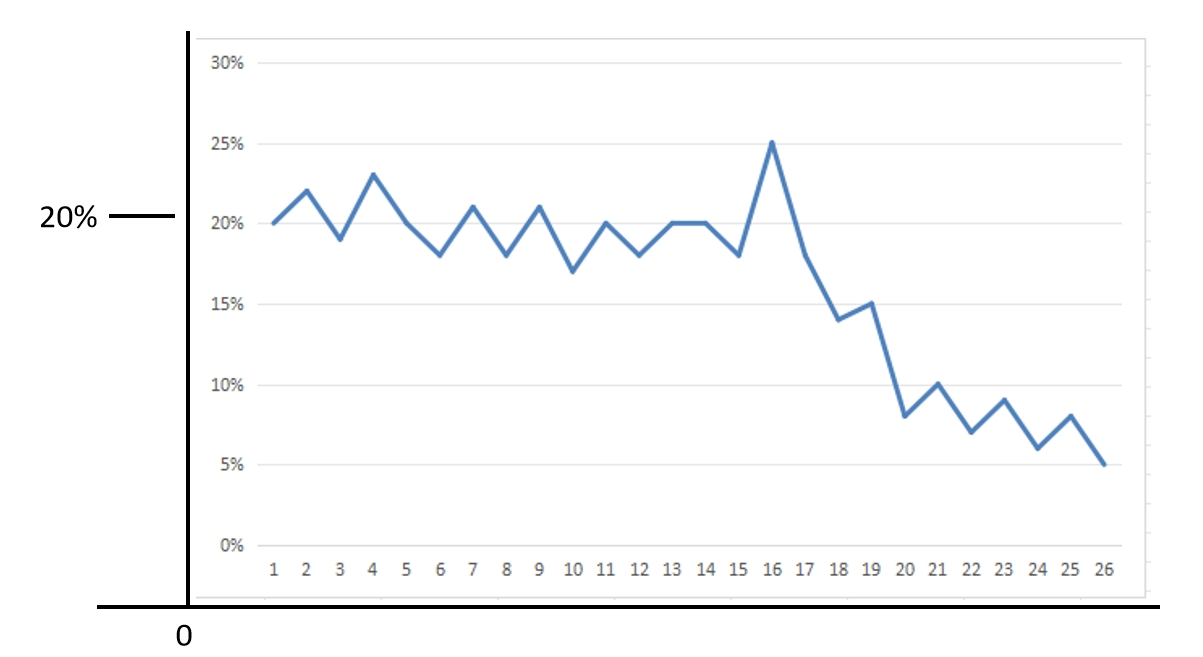
\includegraphics[width=10cm]{微信截图_20241104094040.jpg}

图1-6

所以如果希望敏捷开发有效，不仅仅是走迭代过程，确保进度没偏差，还要确保软件产品质量，也应该用裘兰博士的质量管理思路去看敏捷过程，才能更全面了解如何确保软件开发的质量，控制交付工期。\\
最佳实践，如果没有质量目标、度量衡量和策划，都只是空想，对长远提升企业文化、员工素质没有任何帮助。\\
例如我们想改善团队的策划和估算。首先要识别客户，哪些是主要干系人------甲方有什么要求、内部部门经理有什么要求。然后从他们的诉求变成过程的功能和特征，但如果特征只是描述，没有数字也没有意义，所以要配合可衡量的度量单位，和用什么方式去收集那些数字，然后依据目标定过程要怎么去做，怎样改。例如：

\begin{itemize}
\tightlist
\item
  是否应该从本来的瀑布策划方式制定大的总计划，改用精益的思路，分成迭代
\item
  每次估算应该怎么做、如何监控等
\item
  然后改进过程要不断从实验中优化
\item
  最后还要用数字证明有显著改善，然后在其他团队推广
\end{itemize}

不是单纯``空降''某敏捷流程（例如SCRUM），便能加快团队的发布速度。\\
所以虽然极限编程里每一条实践都是最佳实践，也必须配合质量策划和监控改进才会有效果。\\
乔布斯85年离开苹果，自己开创NEXT公司,他很注重质量，便邀请了裘兰博士(Dr
Juran)从美国东岸飞到西岸，帮他们公司做辅导、改进过程。以下是节录他接受访谈时，对美国企业、质量和裘兰博士的观点：

\framebox{%
\begin{minipage}[t]{0.97\columnwidth}\raggedright
美国已经富裕了很多年。很多企业都忘记要获得成功，还是要关注基本功，包括教育。现在我们美国很多企业面临困难，处处感觉被日本领先了。其实不是日本针对我们，而是我们作为美国企业家应反思一下，为什么我们的战略比日本差，为什么我们的策划不如日本？我们知道裘兰博士多次去日本，帮助日本企业提升质量。现在他回到美国，希望把他的经验带到美国企业，提升竞争力，可以再一次成为世界第一。\\
我觉得裘兰博士很实在，不是泛泛而谈。我们的工程师也深受他这种风格影响。无论我们之中谁问他问题，总裁还是工程师，他都会全心全意用自己的知识解答。所以工程师和我都很希望用他那套方法来做提升。质量提升的道理其实很简单，是一个重复的过程，然后我们需要不断去看，有哪些无效的环节要省略，哪部分要重新设计，不断试验、提升，就这么简单。重点是所有的提升都应该是科学化的，有数据而不是泛泛而谈。\\
一般管理层的思路是：我是领袖，你们应该听我命令。但应该是反过来，让应如何做好的决定权利放在团队手上，做改进不需要请求管理层的批准。改进是工作的一部分，整个架构扁平化，自己管控日常过程，每位工程师应像以前的工匠，愿意花精力不断做好。然后能以自己最后做出的优质工艺、产物自豪。
\strut
\end{minipage}}

从以上丰田故事看到，要有改进必须从高层确定目标出发，再配合一些管理原则和管理者（比如大野耐一总工）的驱动，才可以有效果。员工本身有没有动力也要考虑，但仅仅靠这些还帮不了企业实现真正改进，还需要一些具体的方法和实践，因为所有改进都是由试点项目开始公司的第一小步。\\
对应综合敏捷实践列表，A++除了使用持续改善最底下框里3项和迭代回顾外，也会针对其他3个框讨论：\\
为什么等到客户使用时，才暴露一些很棘手的BUG，但没能预先在内部测试或评审发现？\\
为什么应先写测试用例才开始写代码？\\
为什么不同人估计的故事点差异这么大（超过30\%）？\\
为什么每轮迭代都是最后2-3晚疯狂加班？但还会经常不能按期交付（切割），要延到下一轮?\\
因不少实践已经有很多很好的书籍举例说明，其他如持续集成，结对编程，重构等也会提及，但不会详细讨论。详见表1-2。\\
%\url{文件:敏捷开发实践汇总列表2-2.jpg}

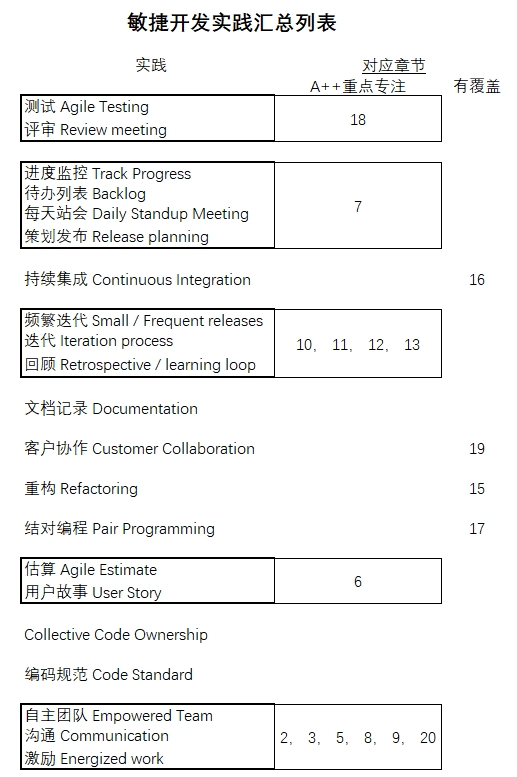
\includegraphics[width=10cm]{敏捷开发实践汇总列表2-2.jpg}

表1-2

\hypertarget{ux7ed3ux675fux8bed}{%
\subsection{结束语}\label{ux7ed3ux675fux8bed}}

若要团队利用敏捷开发帮公司提升没有捷径，只能像乔布斯说的，要达到不断改进的目的就要考虑有没有可靠的数据。因为没数据就没有管理，也不知道现在什么水平，没有标杆，更无法知道几个月后确实有没有改善。所以度量与分析是基础之一。
不是所有公司或者团队都适合做敏捷开发，所以也要考虑公司的文化、管理和团队本身的能力。（2章）\\
很多软件开发团队都缺乏数据，但软件开发与工业生产不一样，很多数据还是要靠个人收集的，例如返工的工作量，所以也要看如何可以把可以让个人开始有收集数据的习惯。（3章、5章）\\
如果个人没有动力，没有好习惯，公司也无法改善。有了这些基础，就可以看团队可以怎么做好估算和计划。（4章、6章、7章）\\
虽然敏捷宣言强调淡化策划，因为它是针对传统的瀑布式开发，一开头做3-6个月的项目计划。但是如果我们把项目拆分成2-4周的迭代，每次迭代还是要做估算和策划。
首先要如何说服高层支持，因为没有高层支持，将过程改进立项，后面肯定不会产生任何效果。（8章）\\
有了高层支持和立项后，改进的过程肯定也不会顺利，因为要改变员工原有的习惯是很难的一件事，而且不会像童话故事一样，挥动一下魔术棒，下个月就立马有效果。（9章）\\
要做好团队的迭代回顾，其实是分析数据，找出根本原因，制定改进方向的最佳时机。（10
- 13章）\\
和前面说的一样，我很同意要做好敏捷开发，不能用SCRUM那种方式，只是针对项目管理做好迭代，还必须要有软件工程的基础。后面我们会从需求一直到产品集成、持续交付等，如何把测试驱动开发这个精益的原则用上。（14
- 20章）\\
市场竞争激烈，单是靠持续改善完善现有的过程，减少缺陷不一定能够支撑公司的长远发展，还是必须要有创新，才有出路。在最后部分会探索个人和公司如何创新。（25
- 27章）\\
在软件开发里，尤其是持续交付、持续集成方面，配置管理起很重要的作用，但因为篇幅有限，我们在本书中暂时不涉及配置管理、版本管理相关的内容。\\
%\url{文件:波波图2024.5.jpg}

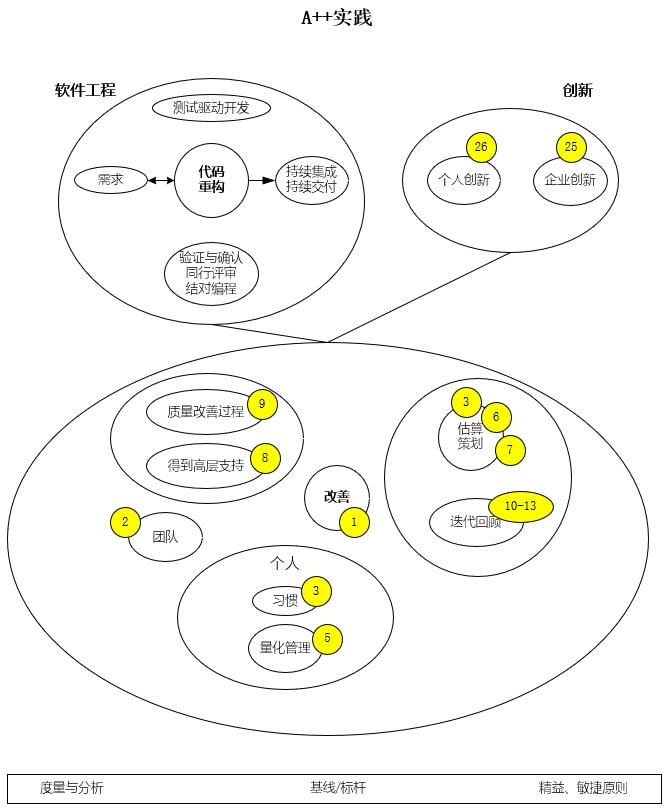
\includegraphics[width=10cm]{波波图20245.jpg}

图1-7

\hypertarget{ux9644ux4ef6}{%
\section{附件}\label{ux9644ux4ef6}}

\hypertarget{ux73b0ux4ee3ux6c7dux8f66ux751fux4ea7}{%
\subsection{现代汽车生产}\label{ux73b0ux4ee3ux6c7dux8f66ux751fux4ea7}}

今天Just-In-Time已成为汽车制造的主流，例如：日产在英国牛津郡(Oxfordshire)专门生产mini车的工厂便能做到：

\begin{itemize}
\tightlist
\item
  从钢材原料到生产出汽车只需要24小时
\item
  整个生产线没有任何中间等候，每68秒出一辆
\item
  每天生产1000辆车
\end{itemize}

%\href{文件:NissanRobots-OIP.h8UAC7FBjlaCmA_mBepJjQHaEi.jpg}{500px}\\

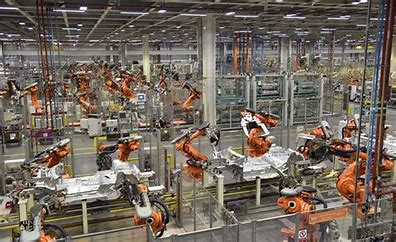
\includegraphics[width=10cm]{NissanRobots-OIPh8UAC7FBjlaCmA_mBepJjQHaEi.jpg}

图1-8

\textbf{挑战}：每一辆汽车都不同------颜色、设备、左右驾驶座等

\begin{itemize}
\tightlist
\item
  生产线上每一辆汽车都按照客户需求订制
\item
  组件不早不晚按需求准时到达生产线
\item
  这便需要信息化系统把客户订单转换成生产信息
\end{itemize}

%\href{文件:微信图片_20240906090104.jpg}{400px}

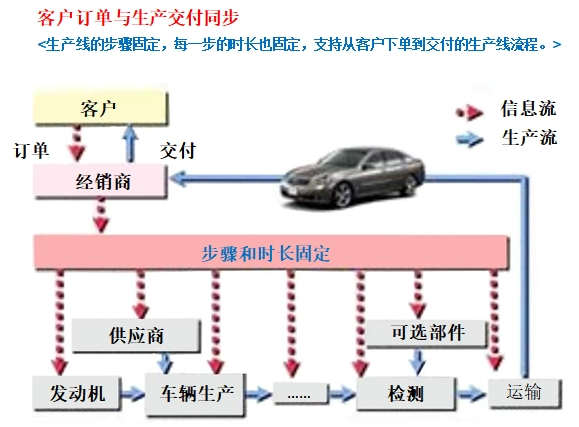
\includegraphics[width=10cm]{微信图片_20240906090104.jpg}

图1-9

例如生产线上每一辆的颜色都可以不同：\\
\href{文件:NissanProdLineOIP.wJFmfMl7q2_V8JaQi4kQ8QHaE6.jpg}{400px}\\

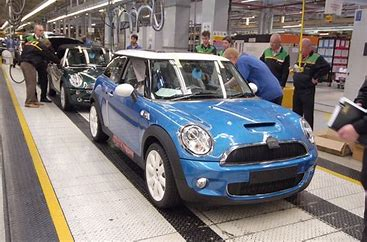
\includegraphics[width=10cm]{NissanProdLineOIPwJFmfMl7q2_V8JaQi4kQ8QHaE6.jpg}

图1-10

\hypertarget{why-ux5b9eux4f8b}{%
\subsection{`` 5 Why ''实例}\label{why-ux5b9eux4f8b}}

大野耐一先生见到生产线上的机器总是停转，虽然修过多次但仍不见好转，便上前询问现场的工作人员。\\
(1W)问：``为什么机器停了？'' 答：``因为超过了负荷，保险丝就断了。''\\
(2W)问：``为什么超负荷呢？'' 答：``因为轴承的润滑不够。''\\
(3W)问：``为什么润滑不够？'' 答: ``因为润滑泵吸不上油来。''\\
(4W)问：``为什么吸不上油来?''答: ``因为油泵轴磨损、松动了。''\\
(5W)问: ``为什么磨损了呢?'' 答:
``因为机器打磨金属零件，空气混进了铁屑等杂质，并掉进机器油缸里。''\\
经过连续5次不停地问``为什么''，找到问题的真正原因（润滑油里面混进了杂质）和真正的解决方案（安装过滤器）。由现象推其本质，因此找到永久性解决问题的方案，这就是5W。

\textbf{针对软件开发的5W例子}：\\
1W：问：为什么显性Bug多？\\
答：开发自测不够。\\
2W：问：为什么开发自测不够？\\
答：1)任务太多，赶着完成;2)只测自己改的Bug，没想到覆盖相关方面。\\
3W：问：为什么要赶着完成任务？\\
答：预留时间本身不足，还有临时任务的加入。\\
4W：问：为什么不能给任务做好估算并预留临时任务时间？\\
答：光做计划中的任务，都完不成，临时任务太多，要不加班，要不简化流程。\\
5W：问：为什么不尽早提出进度滞后的风险，计划没提前同步及随时反馈问题？\\
答：有些计划内容没同步及达成共识，有些任务类型，如，开发自测，没拆解出来或者没明确标准，也没有预留临时任务时间。

措施：计划中关键活动要罗列并明确完成标准；计划不能排太满，预留一部分临时任务的时间；计划要组内同步达成共识。\\

\hypertarget{sux6cd5}{%
\subsection{5S法}\label{sux6cd5}}

本来5S是用于工业生产，例如日本的生产工厂很注重洁净，东西要放在容易找到的固定位置。其实这对生产线员工有很重要的心理作用。如果整个环境都很脏，必然会影响人工做好的动力，如果东西乱放，也容易找不到。5S不仅仅适用于制造业，也适用于服务业，每件东西必须放在固定位置；这也可以用于个人管理，我以前常常在出差去客户现场时，经常忘记把一些东西，如鼠标或插头。但后面我固定了每件东西都应放哪里，临走收拾时就确保那些东西不会遗漏掉。平常工作有一个洁净的环境，也能降低工作压力，提高工作效率。

\href{文件:Screenshot_2023-08-03_211606-1.png}{400px}

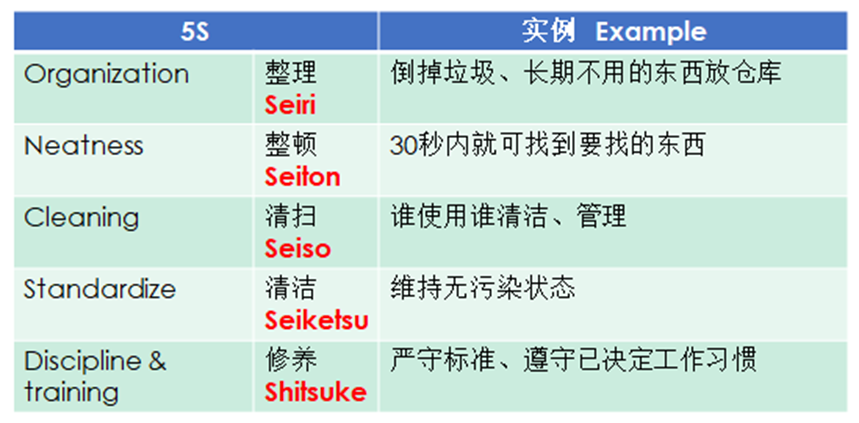
\includegraphics[width=10cm]{Screenshot_2023-08-03_211606-1.png}

表1-3



